\chapter{\IfLanguageName{dutch}{Stand van zaken}{State of the art}}
\label{ch:stand-van-zaken}

% Tip: Begin elk hoofdstuk met een paragraaf inleiding die beschrijft hoe
% dit hoofdstuk past binnen het geheel van de bachelorproef. Geef in het
% bijzonder aan wat de link is met het vorige en volgende hoofdstuk.

% Pas na deze inleidende paragraaf komt de eerste sectiehoofding.

Handschriftherkenning, het woord zegt het zelf al. Het digitalseren van handgeschreven tekst is een veelgebruikte technologie die al sinds de jaren 60 in de maak is en dagelijks talloze transacties automatiseert. Een handgeschreven adres op een brief digitaliseren of fysieke documenten converteren naar een pdf formaat elimineren de nood aan fysieke werkkrachten in verscheidene sectoren en verhogen de efficiëntie. De manier waarop een computertekst transformeert naar zijn digitale tegenligger is niet zo voor de hand liggend en gebruikt in de meeste gevallen een combinatie van technieken die over de jaren heen ontwikkeld werden.
\newline
\newline
Aangezien dit onderzoek de focus legt op tekst extractie, zullen de verscheidene technologieën die handschriftherkenning mogelijk maakt, besproken worden om zo een duidelijk overzicht te geven over wat er precies gebeurt. 
Na deze korte introductie zal het Azure computer Vision framework van Microsoft aangereikt worden. Dit is één van de meer modernere oplossingen die centraal staan bij het praktische gedeelte van dit onderzoek en die het herkennen van handgeschreven teksten vergemakkelijkt.
\section{Optical Character Recognition}
 
OCR (Optical Character Recognition) analyseert de vorm en de complexiteit van een bitsgewijs gemapt karakter en geeft deze vervolgens een waarde. Tegenwoordig kan de meeste OCR software zeer accurate resultaten weergeven als het op machinaal afgedrukte teksten neerkomt. Dit is zeker van toepassing wanneer er een duidelijke font met eenzelfde lengte tussen de karakters gebruikt wordt. \newline \newline Wat echter een groter probleem is dat zich kan voordoen is variabele lengte van karakters, onbekende fonts en al zeker handgeschreven teksten. (\cite{Breithaupt2014}) 



OCR wordt vandaag de dag in een enorm aantal toepassingen gebruikt, zoals het transcriberen van brieven en in zelfrijdende auto's door het herkennen van snelheidslimieten op borden. 

De technologische vordering in dit domein groeit dagelijks en zal in de toekomst enkel maar verbeteren. Echter, de accuraatheid van OCR is verre van perfect en vergt nog altijd een of andere vorm van menselijk toezicht. Op een pagina die 30 karakters telt zal zelfs een dergelijke OCR toepassing met 99 \% accuraatheid, een gemiddelde van 30 fouten maken. Aangezien dit percentage van toepassing is op machinaal geschreven tekst, zal een OCR toepassing losgelaten op handgeschreven tekst een drastisch lager accuraatheidspercentage kennen. (\cite{Nagy1999}) 
\newline \newline
Technieken gebruikt bij het herkennen van handgeschreven woorden maken doorgaans gebruik van holistische of analytische strategieën voor de training en recognition fase. Holistische strategieën maken doorgaans gebruik van een top-down approach voor het herkennen van het volledige woord, hierdoor elimineert men problemen die zich voordoen bij de segmentatie fase. Bij deze strategie worden globale kenmerken van het volledige woord geëxtraheerd en worden vervolgens gebruikt bij herkenning van woorden in een kleine lexicografische omgeving. Analytische strategieën maken gebruik van een bottom-up approach. Expliciete segmentatie van woorden in karakters is nodig voor deze aanpak aangezien deze strategie geïsoleerde karakters herkent. Hierdoor is men niet gelimiteerd door een specifieke lexicografische omgeving maar kan men deze aparte karakters gebruiken in een willekeurige volgorde voor een ongelimiteerd aantal woorden. (\cite{NafizArica2001})

\section{\IfLanguageName{dutch}{Online vs. off-line recognition}{Online vs. off-line recognition}}

Wanneer men spreekt over het effectief herkennen van handgeschreven karakters zijn er 2 technieken die men kan onderscheiden, namelijk \textit{Online Recognition} en \textit{Off-line Recognition}. Online Recognition is een technologie die karakters herkent terwijl men het karakter aan het schrijven is in realtime op een digitaal oppervlak zoals bv. een tablet of een pda toestel.  Input op deze toestellen gebeurt gewoonlijk door middel van een speciale pen die tijdelijke data verzamelt. (\cite{GergelyTimar2003})





De automatische verwerking van karakters bekomt men door de data die de punt van deze pen genereert zoals bv. positie, accelaratie, snelheid. Door middel van de verwerking van deze variabelen kan men de x en y coördinaat van de pen plotten in functie van tijd en hierdoor een karakter traceren (zie Figuur 2.1). (\cite{RejeanPlamondon2000})





De meeste commercieel beschikbare handschriftherkenners lopen 2 tot 3 karakters achter op herkenning. Dit is in principe geen probleem aangezien de gemiddelde persoon tekst schrijft aan een \textbf{1.5-2.5} karakters per seconde. Aangezien realtime translatie van karakters een nogal CPU intensieve taak is wordt door de huidige beschikbare technologieën de lat gelegd op een \textbf{5-10} karakters per seconde. Off-line Recognition wordt tegengesteld van Online Recognition, toegepast op reeds geschreven tekst documenten. (\cite{Tappert1990})  

\begin{figure}[h]
	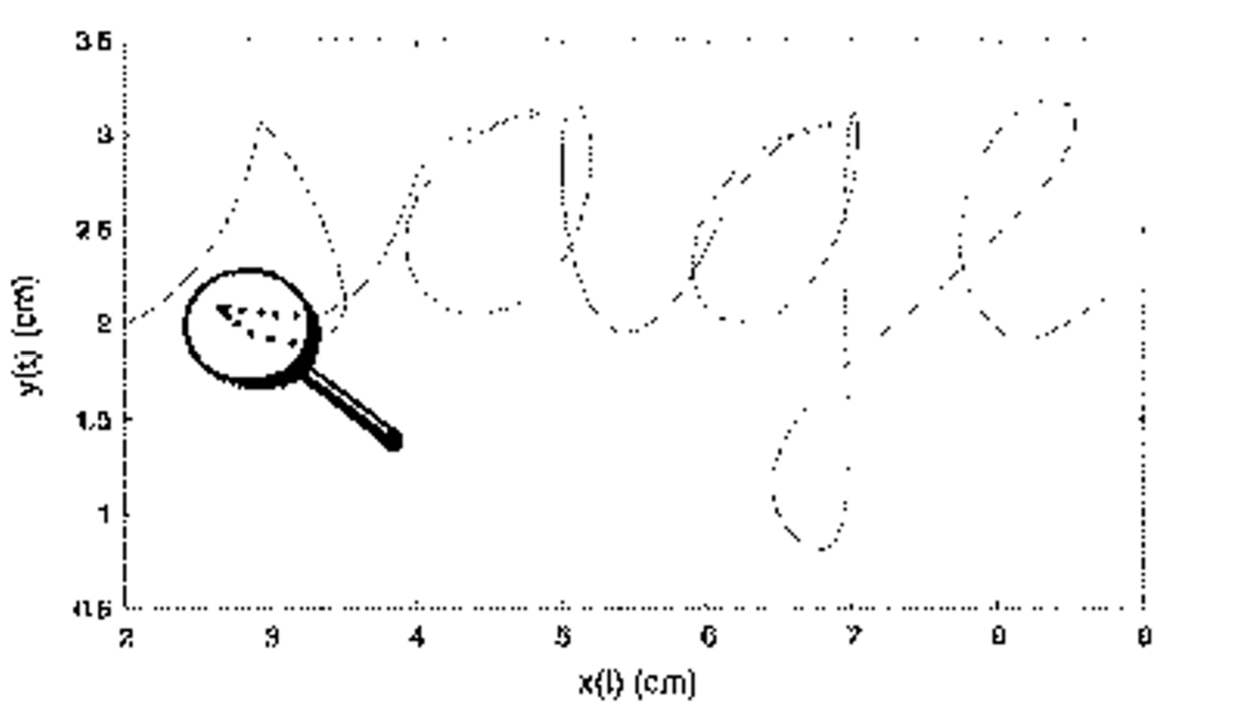
\includegraphics{../../Foto's/Annotation 2020-03-27 163738}
	\caption{x,y coördinaten worden getraceerd in functie van tijd. (\cite{RejeanPlamondon2000})}
	\centering
\end{figure}

Aangezien dit onderzoek primair gebruik zal maken van Off-line Recognition zal dit verder in detail besproken worden.

\section{Off-line recognition}
Het produceren van een performant Off-line Recognition systeem is het doel van tal van onderzoekers in het domein van handschriftherkenning die dit doorheen de jaren proberen te perfectioneren. Handgeschreven teksten zijn een vorm van zelfexpressie, twee dezelfde woorden kunnen een totaal andere betekenis vormen in een verschillende context. Hierdoor kan de achterliggende betekenis van het woord drastisch veranderen. (\cite{GergelyTimar2003})



Zoals reeds besproken maakt Off-line Recognition gebruik van een vooraf geschreven tekst om zo achteraf de tekst te extraheren. Volgens \cite{GergelyTimar2003} kan dit proces dat doorheen verscheidene segmentatie systemen  gebruikt wordt, in een generiek model gegoten worden. 

\begin{figure}[h]
	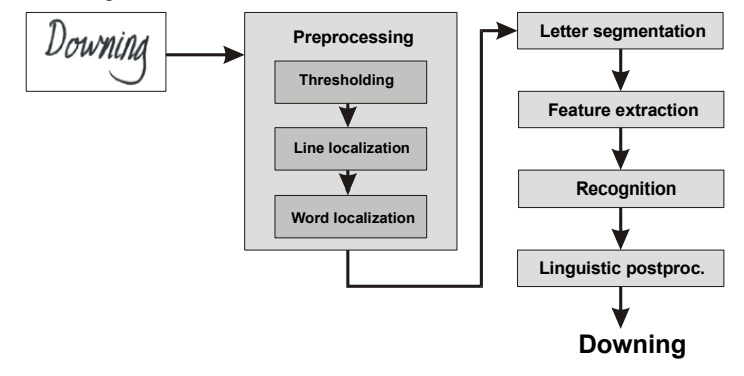
\includegraphics[width=\textwidth,height=\textheight,keepaspectratio]{../../Foto's/Annotation 2020-03-28 141618}
	\captionsetup{justification=centering,margin=2cm}
    \caption{ Het algemeen proces van text extractie via Off-line Recognition. (\cite{GergelyTimar2003})}

	\centering
\end{figure}

\subsection{Preprocessing}

Preprocessing omvat meerdere sub-technieken die toegepast worden vooraleer extractie plaatsvindt. Elk van deze sub-technieken speelt een belangrijke rol in het gehele proces. Zo wordt \textbf{tresholding} toegepast om de effectieve voorgrond-tekst te onderscheiden van de achtergrond. Deze techniek maakt gebruik van een grey-scale versie van het document zodat zwart duidelijk van wit onderscheiden kan worden, zo blijft de tekst geïsoleerd blijft. (\cite{RejeanPlamondon2000}) 

Ter voorbereiding van de karakter segmentatie fase wordt lijn en woordlokalisatie toegepast. Volgens \cite{GergelyTimar2003} helpt deze lokalisatie met het analyseren van de woorden in zijn specifieke context, die op zijn beurt het herkenningspercentage zal verhogen. Het algoritme achter het lokaliseren van deze lijnen is vergelijkbaar met diegene gebruikt in Optical Charachter Recognition. Lijnen worden hierbij gelokaliseerd door het verwerken van de horizontale histogrammen voor het gehele document. Daardoor worden de positie en de graad waar de lijnen een lokaal minimum bereiken gekozen, om zo de plaatsen tussen de lijnen te lokaliseren.  

Eens de lijnen gelokaliseerd zijn kan men vervolgens de woorden lokaliseren. Dit is in principe geen moeilijke taak meer aangezien de onderverdeling van elke lijn gekend is. Men kan door middel van het plaatsen van verticale histogrammen tussen de gekende lijnpunten, de woorden lokaliseren (zie Figuur 2.3). (\cite{GergelyTimar2003}) 

\begin{figure}
\newpage

	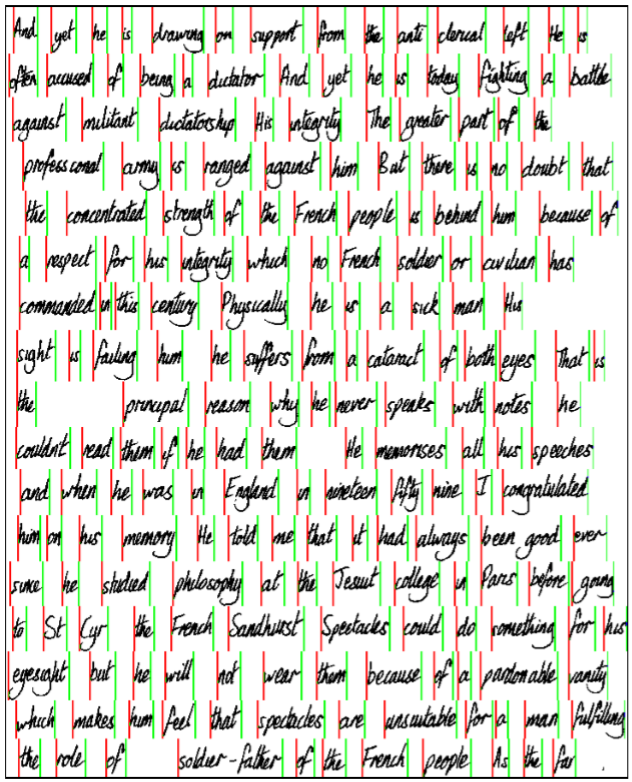
\includegraphics[width=\textwidth,height=\textheight,keepaspectratio]{../../Foto's/line_segmentation_Timar}
	\captionsetup{justification=centering,margin=2cm}
	\caption{Woord segmentatie. (\cite{GergelyTimar2003})}
	\centering
\end{figure}




\subsection{Letter segmentation}
Verdere segmentatie houdt in dat elke letter afgezonderd zal worden. Dit is echter niet zo voor de hand liggend als het lijkt. Het grootste obstakel dat men hier tegenkomt is de variatie in afstand tussen letters. Niet iedereen schrijft letters op dezelfde manier en het kan soms voorvallen dat meerdere karakters overlappen. (\cite{VijayLaxmiSahu2012}) \newline Om karakters op een systematische manier te isoleren wordt Internal Segmentation toegepast. Hierbij probeert men woorden te segmenteren in zijn individuele karakters zonder het gebruik van Feature Extraction. Deze eerste fase houdt geen rekening met eventuele overlappingen en splits elke letter op in een individuele afbeelding. Vervolgens wordt elke afbeelding afzonderlijk geclassificeerd op basis van specifieke kenmerken a.d.h.v. een Hidden Markov Model (HMM).
De cursieve oorsprong van handgeschrift maakt het moeilijk om woorden te segmenteren in karakter afbeeldingen. HMM's helpen om dit probleem op te lossen. 
 (\cite{NafizArica2001}) \newline

HMM’s spelen al jaren een belangrijke rol in het domein van spraak- en gezichtsherkenning. Ondertussen worden deze modellen ook gebruikt bij patroondetectie en vormclassificatie. Deze stochastische modellen kunnen op een zeer efficiënte manier ruis en patroonvariatie in handgeschrift verwerken. Een nadeel van deze aanpak is dat men van de afbeeldingen als invoer verwacht dat deze perfect gesegmenteerd zijn van andere. Aangezien een perfecte aanpak een niet reëel voorkomen is, schat men volgens \cite{Bunke1995} de verwachte herkenningspercentages tussen 74,5 \% en 96.8 \%. 
\subsection{Feature extraction \& Recognition}
Feature extraction is een belangrijk onderdeel van elk patroonherkenning systeem. Dit proces wordt uitgevoerd om de belangrijkste data te extraheren uit de ruwe dataset. Het uiteindelijke doel van dit proces is om een lijst van specifieke “features” van de karakters te bekomen. Met deze aanvullende data kan men vervolgens de herkenningspercentages maximaliseren. Zoals eerder aangereikt verschilt de variëteit in handgeschreven karakters drastisch en kan het extraheren van deze “features” een complexe taak zijn. (\cite{VijayLaxmiSahu2012}) \newline  \newline Men kan karakter features onderscheiden in twee types, namelijk statistische en culturele. Een voorbeeld van statistische feature extraction is Zoning, waarbij men elke karakter afbeelding opdeelt in NxM zones. Hierdoor bekomt men bij bv. een afbeelding van 90 x 60 pixels een onderverdeling van 54 gelijke zones. Vervolgens wordt dit proces herhaald voor elke afbeelding van eenzelfde karakter. Men verkrijgt hierdoor een subset van karakter features waarvan het gemiddelde genomen kan worden. Dit gemiddelde vormt één enkele feature waarde die telkens in die zone geplaats kan worden. (\cite{VijayLaxmiSahu2012})  

Uiteindelijk worden deze features verstuurd naar de recognition engine. Deze retourneert vervolgens een lijst van woorden elk respectievelijk met zijn vertrouwensniveau. Dit niveau stelt voor hoe zeker het algoritme is van zijn voorspelling. (\cite{GergelyTimar2003})

\section{Machine Learning (ML)}
Aangezien in de volgende hoofdstukken machinaal leren aan bod komt, zal hier een kleine inleiding op gegeven worden. 

Machinaal leren (ML) is een concept waarbij men data en een algoritme samen brengt om een specifiek probleem op te lossen. Eens de data en het algoritme getraind zijn krijgt men een model als output. Dit model kan men opnieuw gebruiken met andere data. Het getrainde model geeft inzicht gebaseerd op de nieuwe data. Het bouwen van een ML systeem vergt enige kennis van data science en ML. (\cite{Microsoft2020e})



Volgens \cite{SalimAlHabsib2019} kan men machinaal leren aanpakken op drie manieren: gesuperviseerd leren, ongesuperviseerd leren en semi-gesuperviseerd leren. Gesuperviseerd leren maakt gebruik van gelabelde trainingsdata. Het labelen van deze data neemt zowel tijd als geld in beslag, maar kan op zijn beurt weer geautomatiseerd worden door een neuraal netwerk.  



Semi-gesuperviseerd leren wordt volgens \cite{Zhu2005} beschreven als een speciale vorm van classificatie. Zoals reeds aangereikt, kan gesuperviseerd leren een ingewikkelde en dure manier zijn om een classificatie algoritme op te bouwen. Het labelen van data heeft in de meeste gevallen een vorm van menselijke controle nodig om een acceptabel resultaat te bekomen. Semi-gesuperviseerd leren lost dit probleem op door gebruik te maken van een grote hoeveelheid ongelabelde data, gepaard gaande met een deel gelabelde data. Een vergelijkbare toepassing hiervan, kan men terugvinden bij de Custom Vision service van Azure Cognitive Services. Ongesuperviseerd leren maakt gebruik van ongelabelde data. Het classificeren gebeurt hier door het clusteren van data met gelijkaardige patronen. 

\subsection{Neurale netwerken}

\cite{Kumar2016} beschrijft een  artificieel neuraal netwerk , als een krachtige modelleer tool, die complexe in- en uitgaande relaties kan weergeven en opvangen. De motivatie voor de ontwikkeling van neurale netwerken, stemt af van de nood aan een systeem dat complexe en intelligente taken kan uitvoeren, net zoals de taken uitgevoerd door het menselijk brein. Neurale netwerken komen op twee manieren overeen met het menselijk brein. Ze vergaren leerstof door het leren van vorige transacties en de vergaarde leerstof wordt opgeslagen in de vorm van synaptische gewichten.   


Volgens \cite{Microsoft2020d} worden de volgende types ANN als populairst beschouwd:

\subsubsection{Feedforward neuraal netwerk (FNN)}
Een FNN is één van de meest eenvoudige soort artificiële neurale netwerken. In een FNN mag data maar één richting vloeien, namelijk van de input laag naar de output laag. Data wordt getransformeerd door het gebruik van meerdere lagen. Elke laag bestaat uit een aantal neuronen en is volledig geconnecteerd met al de neuronen in de voorgaande laag. \newpage De laatste volledig geconnecteerde laag stelt de output voor en eveneens de voorspelde labels. (\cite{Microsoft2020d})

\subsubsection{Recurrent neuraal netwerk (RNN)}
Recursieve neurale netwerken worden in een aantal specifieke domeinen gebruikt. Dit type netwerk slaagt de output van een laag op en geeft deze vervolgens terug aan de input laag. Hierdoor bekomt men een vorm van recursie en kan men de uitkomst van een laag op voorhand voorspellen. Deze netwerken worden voornamelijk gebruikt voor complexe taken zoals handschriftherkenning en taalherkenning. (\cite{Microsoft2020d})  
\subsubsection{Convolutioneel neuraal netwerk (CNN)}
Convolutionele neurale netwerken zijn één van de meest doeltreffende types van netwerken, gepaard met een unieke architectuur. Lagen worden in 3 dimensies opgebouwd: breedte, hoogte en diepte. 

Neuronen in de ene laag connecteren partieel met al de neuronen in de volgende laag. De finale output laag wordt gereduceerd tot een enkelvoudige vector van waarden die het vertrouwensniveau van de voorspelling weergeeft. Convolutionele neurale netwerken worden voornamelijk gebruikt bij video en afbeelding herkenning. (\cite{Microsoft2020d}) 






\section{Cloud computing providers}
Wanneer men dus uiteindelijk handschriftherkenning in een project wenst te integreren zijn er meerdere mogelijkheden. Men kan gebruik maken van een Cloud computing platform dat services zoals tekstherkenning en extractie aanbiedt, maar er is natuurlijk ook de optie om een open source framework zoals Tenserflow of Theano te gebruiken. Bij deze open source optie wordt er verwacht dat men het neurale netwerk/model volledig zelfstandig opbouwt en een eigen inbreng van trainingsdata voorziet. In sommige gevallen kan dit een voordeel zijn, wanneer er bv. een zeer specifiek model nodig is. Cloud gebaseerde oplossingen hebben hierbij het voordeel dat ze een model gebruiken dat getraind is met data verzameld door de provider. Verscheidene providers laten het toe om zelf nog extra trainingsdata in te brengen in het model, zoals bv. de Custom Vision service van Microsoft Azure. 



In het domein van Cloud Computing zijn er dus enkele marktleiders die een forse voorsprong hebben door middel van de hoeveelheid data die zij door de jaren heen hebben verzameld. Dit onderzoek maakt voornamelijk gebruik van de services die Microsoft Azure te bieden heeft, maar er zullen in de volgende hoofdstukken nog enkele andere alternatieven besproken worden die een gelijkaardig pakket aanbieden. 

\section{\IfLanguageName{dutch}{Microsoft Azure}{Azure}}

Microsoft Azure is een uitgebreide set van cloud services die helpt bij het organiseren en het aanpakken van uitdagingen die zich voordoen op grootschalige niveaus. Deze uitdagingen worden typisch gerealiseerd door middel van cloud computing.  Wanneer iemand niet beschikt over de nodige server of opslagcapaciteiten die zich kunnen voordoen bij sommige uitdagingen, dan kan men opteren voor cloud computing.  Hierbij kan men bij providers zoals Azure, gebruik maken van de cloud om data op te slagen. Cloud computing platformen zoals Azure worden gerealiseerd door meerdere datacentrales op een globaal niveau. Hierdoor kan men wereldwijd op een betrouwbare manier toegang bieden tot verscheidene services die beschikbaarheid en betrouwbaarheid van data realiseren. (\cite{Microsoft2020a}) \newline
\newline
Volgens \cite{VaibhavAGhandi1999} kan men cloud computing opdelen in verschillende service modellen. 





\subsection{Software as a Service (SaaS)}
Software as a Service is een software gedistribueerd model waarin applicaties door een service provider gehost worden. De betalingsmethode voor SaaS volgt een subscriptie gebaseerd model. Hierdoor kunnen organisaties de focus leggen op hun core business zonder zich bezig te houden met infrastructuur management. (\cite{ManishGodse2009})
\subsection{Platform as a Service (PaaS)}
Platform as a Service biedt bedrijven een digitaal platform voor ontwikkeling en inzet van hun eigen applicaties en services. Hierdoor elimineert men de nood aan het onderhouden van servers, het programmeren van software en het opstellen van interne veiligheid protocollen. (\cite{Wright2019})
\subsection{Infrastructure as a Service (IaaS)}
Infrastructure as a service is de bundeling van hardware en geassocieerde software geleverd als een service. Deze hardware kan bestaan uit servers, opslag en of netwerk toepassingen. Meegeleverde software kan gaan van besturingssystemen, virtualisatie technologieën of file systemen. Bij IaaS is de provider enkel verantwoordelijk voor het operationeel houden van de data centers. Klanten zijn zelf verantwoordelijk voor het opstellen en het onderhouden van hun software services. (\cite{Bhardwaj2010})
\begin{figure}[h]

	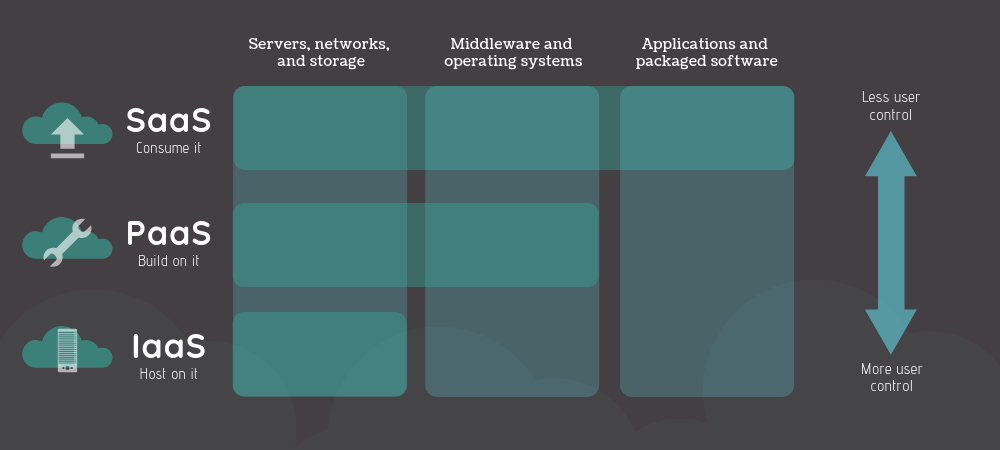
\includegraphics[width=\textwidth,height=\textheight,keepaspectratio]{../../Foto's/Cloud-Models-Graphics}
	\captionsetup{justification=centering,margin=2cm}
	\caption{SaaS,IaaS,PaaS. (\cite{Wright2019})}
	\centering
\end{figure}
\section{\IfLanguageName{dutch}{Azure Cognitive Services}{Azure Cognitive Services}}
Azure cognitive services geeft ontwikkelaars de kans om op een eenvoudige wijze artificiële intelligentie toe te voegen aan hun project zonder enige voorkennis te hebben van machinaal leren en/of data science. Toepassingen van cognitive services gaan van het analyseren en herkennen van objecten in afbeeldingen tot het herkennen van emoties op gezichten in realtime.  Een cognitive service levert deels of de volledige componenten die nodig zijn in een toepassing die gebruik maakt van machinaal leren. Deze componenten kunnen bestaan uit bv. data, het algoritme of een vooraf getraind model. Een service zoals deze verwacht dat de gebruiker generieke info over de dataset meelevert.  (\cite{Microsoft2020b}) \newline \newline



Azure cognitive services kan geclassificeerd worden als een Software as a Service (SaaS), omvat een groep van services die onmiddellijk beschikbaar zijn voor deployment en kunnen opgedeeld worden in de volgende categorieën:

\begin{itemize}
	\item \textbf{Decision:} Bouwt apps die aanbevelingen geven voor het maken van efficiënte en geïnformeerde beslissingen.
	\item \textbf{Language:} Zorgt ervoor dat men taal kan verwerken met voorgebouwde scripts, die emoties evalueren en leren wat een gebruiker juist wenst.
	\item \textbf{Search:} Voegt Bing Search API’s toe aan apps en geven de mogelijkheid om miljarden webpagina’s, afbeeldingen en video's te doorzoeken met één enkele API.
	\item \textbf{Speech:} Transformeert gesproken tekst naar digitale tekst en vertaalt één taal naar een ander samen met spraak verificatie en herkenning.
	\item \textbf{Vision:} Herkent, identificeert, indexeert en onderhoudt foto's, video's en digitale inkt toepassingen.
\end{itemize}
Sommige van deze services maken het mogelijk om zelf training data mee te geven om vervolgens een model te trainen. Hierdoor kan men het model uitbreiden door gebruik te maken van de data die de service levert samen met de data die de gebruiker meelevert. Wanneer men zelf data meelevert, kan het voorvallen dat deze data nog op een specifieke manier gelabeld moet worden conform met de service. Door zelf data mee te geven kan je de service vormen naar de noden van de gebruiker. (\cite{Microsoft2020b})



\section{\IfLanguageName{dutch}{Azure Computer Vision framework}{Azure Computer Vision framework}}
Computer vision biedt een aantal services die afgedrukte of handgeschreven tekst detecteren en extraheren. Dit kan in verschillende situaties toegepast worden, zoals het maken van notities, inscannen van medische dossiers of bij beveiliging en bankieren. Voor het herkennen van tekst levert het Computer Vision Framework drie verschillende API’s elk geoptimaliseerd voor een specifieke toepassing. (\cite{Microsoft2020c})

\subsection{Read API}
De Read API kan tekst in een afbeelding detecteren met behulp van de nieuwste herkenningsmodellen van computer vision, en zet geïdentificeerde tekst om in een karakterstroom. Deze API is voornamelijk geoptimaliseerd voor afbeeldingen die veel tekst hebben of
met een bepaald aantal visuele ruis. Voor elke lijn tekst wordt eveneens beslist welk herkenningsmodel gebruikt zal worden. Hierdoor ondersteunt de API geprinte en handgeschreven tekst. De Read API voert de herkenningsalgoritmen asynchroon uit omdat men bij data intensieve documenten een langere tijd nodig heeft tot men een resultaat verkrijgt. (\cite{Microsoft2019})
\newline
\newline
De leesoperatie houdt de originele lijn groeperingen van herkende woorden bij in zijn output. Elke lijn heeft zijn eigen coördinaten. Respectievelijk heeft elk woord in deze lijn ook zijn specifieke coördinaten. Wanneer een herkend woord een lage vertrouwens niveau heeft wordt dit percentage per woord meegeleverd. (\cite{Microsoft2019})
\subsection{OCR API}
Men kan in grote lijnen de OCR API gelijkstellen aan de Read API, echter voert deze API zijn operaties synchroon uit en zijn deze niet geoptimaliseerd voor data intensieve documenten. Hiervoor maakt de OCR API gebruik van een ouder herkenningsmodel maar is deze ook compatibel met meerdere talen. 

Wanneer nodig kan OCR de rotatie van specifiek herkende tekst aanpassen door middel van de afbeelding te draaien op zijn horizontale as (ziet figuur 2.5).  
\begin{figure}[h]
	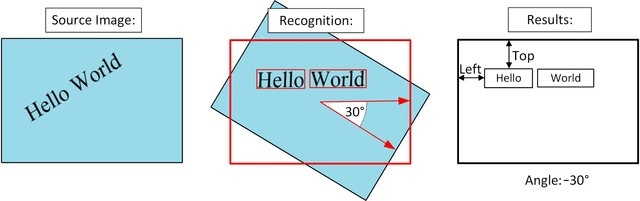
\includegraphics[width=\textwidth,height=\textheight,keepaspectratio]{../../Foto's/vision-overview-ocr}
		\captionsetup{justification=centering,margin=2cm}
	\caption{Rotatie correctie van een woord via de OCR API. (\cite{Microsoft2019})}
	\centering
\end{figure}
\subsection{Recognize text API}
De Recognize Tekst API is in zekere zin gelijkaardig aan dat van OCR, maar verwerkt zijn operaties asynchroon en maakt gebruik van geüpdatete herkenningsmodellen. Deze API heeft echter enkele limitaties. De accuraatheid van deze operaties is grotendeels afhankelijk van de kwaliteit van de gebruikte afbeeldingen. De volgende factoren kunnen de accuraatheid beïnvloeden: 
\begin{itemize}
	\item Wazige afbeeldingen.
	\item  Handgeschreven of cursieve tekst.
	\item Artistieke font keuzes.
	\item Kleine tekstgrote.
	\item Complexe achtergronden, schaduwen over tekst.
\end{itemize}
(\cite{Microsoft2019})


\section{\IfLanguageName{dutch}{Google Cloud Platform (GCP)}{Google}}
Google Cloud Platform (GCP) biedt net zoals Microsoft Azure services voor opslag, analyse, big data en machine learning op een globaal niveau. Google realiseert dit door hun grootschalig netwerk van datacenters verspreid over 22 regio’s. Door de spreiding van deze locaties kan men efficiënte en betrouwbare connectie met de cloud verzekeren. 


Men kan de services die Google levert opdelen in enkele omvattende categorieën:
\begin{itemize}
	\item \textbf{Compute engine:} De compute engine levert flexibele virtuele machines die draaien op de Google datacenters. 
	\item \textbf{Storage \& Databases:} Voorziet globale toegang tot verschillende opslag architecturen op enterprise niveau.  
	\item \textbf{Machine learning:} Maakt het mogelijk voor developers om machine learning in een project te integreren en eveneens over te gaan naar een productieomgeving.  \newpage
	\item \textbf{Big data:} Opslag en analyse mogelijkheden van grote hoeveelheden data, gepaard met data warehouse integratie en stream analytics. 
	\item \textbf{Developer tools:} Voorziet pipelines en automatisatie van deployment in een productie omgeving.
	
\end{itemize}
\begin{figure}[h]
	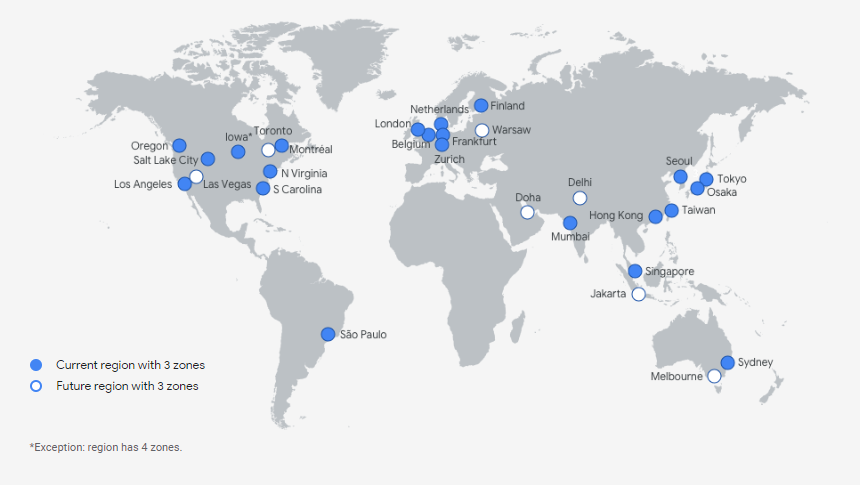
\includegraphics[width=\textwidth,height=\textheight,keepaspectratio]{../../Foto's/Google cloud locations}
		\captionsetup{justification=centering,margin=2cm}
	\caption{Google datacenters. (\cite{Google2020a})}
	\centering
\end{figure}


Vergelijkbaar met Azure Cognitive Services heeft GCP een gelijkaardig machine learning platform, namelijk AI hub. De Google Cloud AI Hub is een gehoste opslagplaats waarbij men kant-en-klare AI toepassingen kan implementeren, en end-to-end AI pipelines kan opzetten. AI Hub biedt ook professionele deelmogelijkheden waarmee men AI toepassingen privé kan hosten. (\cite{Google2020b})



Naar aanleiding van dit onderzoek worden meerdere toepassingen besproken waarmee handschriftherkenning gerealiseerd kan worden. De oplossing die Google hier namelijk voor voorziet is Google Vision AI, meer specifiek de Cloud Vision API. 

Google Vision AI biedt meerdere opties aan om computer visie modellen te integreren in applicaties of in websites. Men kan deze opties verder onderverdelen in drie categorieën: 
\begin{itemize}
	\item Auto ML Vision
	\item Cloud Vision API
	\item Cloud Vision product search
\end{itemize}
(\cite{Google2020c})


\subsection{Cloud Vision API}
De Google Cloud Vision API biedt een verzameling van technologieën die men kan gebruiken om de inhoud van afbeeldingen te analyseren. Hiervoor kan men gebruik maken van een zelf getraind ML model of één van de vele vooraf getrainde modellen die de API aanbiedt. Door gebruik te maken van AutoML Vision kan men naast de vooraf gedefinieerde labels, zelf specifieke labels toevoegen. Hierdoor kan men een domein specifiek model opbouwen. Toepassingen die gebruik maken van deze vooraf getrainde modellen omvatten, maar zijn niet gelimiteerd tot: afbeelding classificatie, object detectie, geprinte en handgeschreven tekstherkenning, gezichtsherkenning, product logo identificatie. (\cite{Google2020d})


De Vision API kan tekst in afbeeldingen detecteren en extraheren. Net zoals het Computer Vision framework van Microsoft, maakt Google ook gebruik van de OCR technologie om de achterliggende logica van karakter herkenning te realiseren. Er zijn namelijk 2 annotatie technieken die de Vision API ondersteunt: 

\begin{itemize}
	\item \textbf{TEXT\_DETECTION:} Deze annotatie techniek wordt voornamelijk gebruikt voor het extraheren van geprinte tekst. Hiermee kan men bv. de tekst van een verkeersbord herkennen.  
	\item \textbf{DOCUMENT\_TEXT\_DETECTION:} Wordt ook gebruikt voor tekst extractie maar is geoptimaliseerd voor documenten en handgeschreven teksten. 
\end{itemize}


Beide technieken worden getriggerd bij aanvang van een REST request. De request body bestaat uit een JSON string. In deze string wordt een base64 gecodeerde afbeelding meegegeven samen met de gewenste annotatie techniek. Wanneer de request als succesvol wordt beschouwd door de server, dan retourneert deze een HTTP status code 200 OK. 


De status code 200 geeft aan dat het verzoek geslaagd is, gepaard met deze status code wordt ook een response body geretourneerd in JSON formaat. In deze response wordt de gedetecteerde zin meegegeven, de geschatte taal en de coördinaten van waar de zin zich precies bevindt in de afbeelding. De Vision API voorziet ook de optie om rechtstreeks een afbeelding van Google Cloud of het web mee te geven bij de request. (\cite{Google2020e}) 


Op figuur 2.7 ziet men een voorbeeld van hoe een JSON request body opgebouwd wordt. 


Beide types ondersteunen de integratie van één of meerdere taal hints. Deze hints specifiëren de taal van de tekst die voorkomt in de meegegeven afbeelding. Dit kan in de sommige gevallen de snelheid van extractie verhogen. Meestal wanneer men dit niet specifieert bekomt men betere resultaten, aangezien de API zelf automatisch de taal detecteert. Het kan zelfs voorvallen dat een foutieve taal hint de herkenning kan hinderen. 
\begin{figure}[h]
	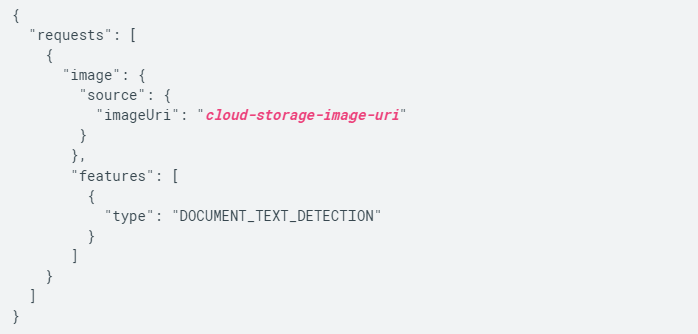
\includegraphics[width=\textwidth,height=\textheight,keepaspectratio]{../../Foto's/vision OCR request body Google}
		\captionsetup{justification=centering,margin=2cm}
	\caption{Text extractie request body. (\cite{Google2020e})}
	\centering
\end{figure}

\section{Amazon Web Services (AWS)}
Amazon Web Service (AWS) is de derde grote tegenhanger in het domein van Cloud Computing, naast Microsoft Azure en Google Cloud.  



AWS maakt hun services wereldwijd beschikbaar op meerdere locaties. Deze locaties bestaan uit verschillende individuele regio's en zones. Elke regio is verder opgedeeld in geïsoleerde locaties gekend als “beschikbaarheid zones”. AWS laat het toe om meerdere resources zoals instanties van AWS services of data, te deployen op meerdere locaties. Deze resources worden niet over verschillende regio's gedupliceerd, tenzij men dit expliciet specifieert. Elke regio is volledig zelfstandig en isoleert zich volledig van andere regio’s. Hierdoor bekomt men een hoge graad van fout tolerantie en stabiliteit over het netwerk. (\cite{Amazon2020a})



AWS levert net zoals de concurrentie, tal van Cloud Computing services. Elk van deze service kan gebundeld worden in een cluster van services: 


\begin{itemize}
	\item \textbf{Analytics}
	\item \textbf{Application Integration}
	\item \textbf{Compute}
	\item \textbf{Database}
	\item \textbf{Internet of Things}
	\item \textbf{Machine Learning}
	\item \textbf{Containers}
\end{itemize}


\subsection{Amazon Rekognition}
Amazon Rekognition valt onder de AWS Machine Learning cluster maakt het mogelijk om op een eenvoudige wijze video en afbeelding analyse toe te voegen aan een applicatie. Wanneer men een afbeelding of een video meegeeft in een extractie request naar de Rekognition API, dan kan de API op een accurate manier objecten, mensen, tekst en activiteiten detecteren. Er is ook de mogelijkheid om net zoals bij Google Cloud Vision, custom labels mee te geven, om een model te maken dat gespecifieerd is aan de noden van de klant. (\cite{Amazon2020b})


De Rekognition API kan tekst in afbeeldingen en video's detecteren, en deze vervolgens converteren naar machinale tekst. Men kan een afbeelding aan een request meegeven in de vorm van een base64 gecodeerde string of een Amazon S3 object (zie figuur 2.8). Amazon S3 is een opslag service aangeboden door AWS, waar men key–value paren van objecten in kan opslagen. Deze objecten kan men rechtstreeks meegeven aan een API request en is niet gelimiteerd tot enkel afbeeldingen. (\cite{Amazon2019})

\begin{figure}[h]
	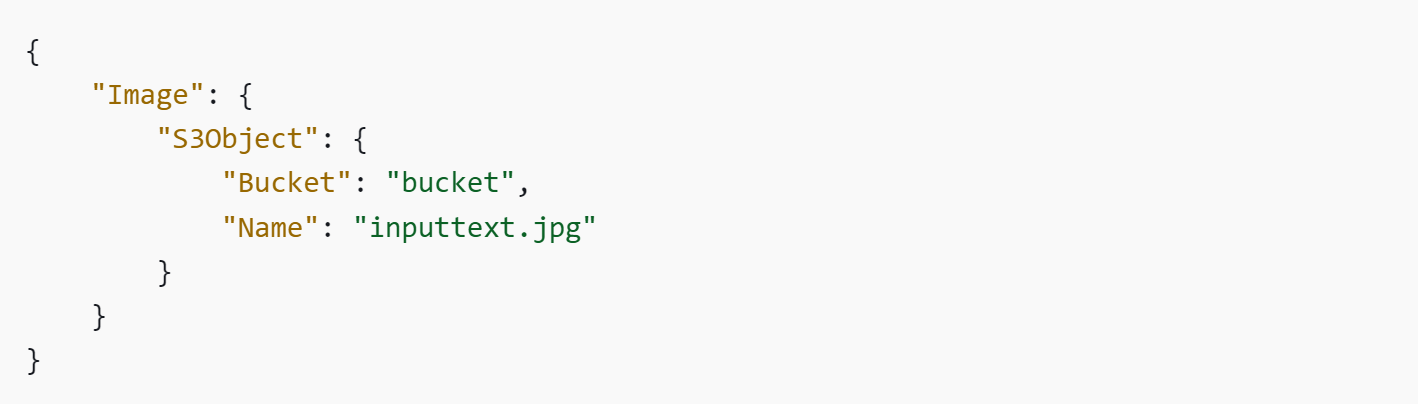
\includegraphics[width=\textwidth,height=\textheight,keepaspectratio]{../../Foto's/AWS text detection request}
	\captionsetup{justification=centering,margin=2cm}
	\caption{Text extractie request body. (\cite{Amazon2019})}
	\centering
\end{figure}



Vervolgens retourneert de API een JSON response waarin de herkende woorden samen met hun vertrouwensniveau en positie weergeven worden. 

\section{Eerder uitgevoerd onderzoek}
Zoals aangereikt in de inleiding is dit onderzoek gebaseerd op een recent onderzoek uitgevoerd door Vectr. Consulting in samenwerking met de Christelijke Mutualiteit. Hierbij ontwikkelde zij een bot die automatisch doktersgeschrift op Belgische doodsaktes met een accuraatheid van 47 \% correct voorspelde. Hiervoor maakten zij gebruik van het machine learning framework Tenserflow van Google, gepaard met een convolutioneel neuraal netwerk ontwikkeld door H. Scheidl. De data gebruikt in het trainen van dit neuraal netwerk werd verzameld gedurende 6 jaar. Finale resultaten van dit onderzoek tonen aan dat 47\% van de testset correct gelabeld werd door het neuraal netwerk. Dit percentage is zeer gevoelig aan de kwaliteit van de preprocessing op de data en de segmentatie van woorden in karakters. Uit dit onderzoek kon men uiteindelijk concluderen dat het herkennen van doktersgeschrift zeker haalbaar is met een degelijk getraind neuraal netwerk. 

